% !TEX TS-program = pdflatex
\documentclass[11pt]{article}

% -------------------- Packages --------------------
\usepackage[a4paper,margin=1in]{geometry}
\usepackage{amsmath,amssymb}
\usepackage[T1]{fontenc}
\usepackage{lmodern}
\usepackage{xcolor}
\usepackage{tcolorbox}
\tcbuselibrary{skins,breakable}
\usepackage{enumitem}
\usepackage{hyperref}

% --- Tables & Diagrams ---
\usepackage{booktabs}
\usepackage{array}
\usepackage{colortbl}
\usepackage{tikz}
\usetikzlibrary{arrows.meta,calc}
\usepackage{pgfplots}
\pgfplotsset{compat=1.18}

\pagestyle{empty}

% -------------------- Dark Theme Colors --------------------
\definecolor{bg}{HTML}{000000}
\definecolor{pairbg}{HTML}{121212}
\definecolor{solbg}{HTML}{0A0A0A}
\definecolor{border}{HTML}{2A2A2A}
\definecolor{text}{HTML}{FFFFFF}
\definecolor{muted}{HTML}{C9CDD3}
\definecolor{gold}{HTML}{FFD700}
\definecolor{green}{HTML}{4ADE80}
\definecolor{cyan}{HTML}{38BDF8}
\definecolor{redacc}{HTML}{F87171}

\definecolor{tablehead}{HTML}{1B1B1B}
\definecolor{tablerow}{HTML}{101010}

\pagecolor{bg}
\color{text}

\hypersetup{
  colorlinks=true,
  linkcolor=cyan,
  urlcolor=cyan
}

\setlength{\parindent}{0pt}
\setlength{\parskip}{10pt}

\setlist[itemize]{left=1.4em,itemsep=6pt,topsep=6pt}
\setlist[enumerate]{left=1.6em,itemsep=4pt,topsep=4pt}

% -------------------- tcolorbox Base --------------------
\tcbset{
  enhanced,
  breakable,
  arc=12pt,
  boxrule=0.8pt,
  left=16pt,right=16pt,top=12pt,bottom=12pt
}

% FIX: remove default (orange) title styling by explicitly setting title background + title text color
\newtcolorbox{QAPair}[1]{%
  colback=pairbg,
  colbacklower=solbg,
  colframe=border,
  coltext=text,
  colbacktitle=tablehead,
  coltitle=gold,
  title=\bfseries #1,
  fonttitle=\bfseries,
  segmentation style={draw=border, dashed, line width=0.6pt},
}

\newtcolorbox{QuickBox}{%
  colback=pairbg,
  colframe=cyan,
  coltext=text,
  colbacktitle=pairbg,
  coltitle=cyan,
  fontupper=\color{text},
  borderline north={4pt}{0pt}{cyan},
  arc=14pt,
  boxrule=0.8pt
}

% Helper for step headings
\newcommand{\Step}[1]{\textcolor{muted}{\textbf{Step #1:}}}

% -------------------- pgfplots dark styling --------------------
\pgfplotsset{
  every axis/.append style={
    axis line style={color=text},
    tick style={color=text},
    ticklabel style={color=text},
    label style={color=text},
    title style={color=text},
    grid style={color=border},
    legend style={draw=border, fill=pairbg, text=text},
  }
}

% A small helper to format tables nicely on dark background
\newcommand{\DarkTable}{%
  \rowcolors{2}{tablerow}{solbg}
  \renewcommand{\arraystretch}{1.2}
  \setlength{\tabcolsep}{10pt}
}

% --------- Small helper: plot one complex point on Argand plane ----------
\newcommand{\PointPlot}[4]{% label, x, y, axisrange
\begin{center}
\begin{tikzpicture}
\begin{axis}[
  axis lines=middle,
  grid=both,
  xmin=-#4, xmax=#4,
  ymin=-#4, ymax=#4,
  width=0.70\linewidth,
  height=6.0cm,
  xlabel={Re},
  ylabel={Im},
  axis equal image,
]
\addplot+[only marks, mark=*, mark size=2.4pt, color=cyan] coordinates {(#2,#3)};
\node[anchor=south west, text=text] at (axis cs:#2,#3) {$#1(#2,#3)$};
\end{axis}
\end{tikzpicture}
\end{center}
}

% --------- Helper: vector from origin (for sum/diff) ----------
\newcommand{\VectorFromOrigin}[3]{% x,y,label
\addplot+[->, thick, color=cyan] coordinates {(0,0) (#1,#2)};
\node[anchor=south west, text=text] at (axis cs:#1,#2) {$#3$};
}

% ============================================================
\begin{document}

\begin{center}
{\LARGE\bfseries \textcolor{gold}{Exercise 1.2 --- Complex Numbers (Solutions)}}\\[-2pt]
\end{center}

\begin{QuickBox}
{\color{cyan}\bfseries Quick formulas (Complex Numbers)}\par\medskip
\begin{itemize}
\item \textbf{Additive inverse:} If $z=a+bi$, then $-z=-a-bi$ and $z+(-z)=0$.
\item \textbf{Conjugate:} $\overline{a+bi}=a-bi$.
\item \textbf{Modulus:} $|a+bi|=\sqrt{a^2+b^2}$.
\item \textbf{Key identity:} $(a+bi)(a-bi)=a^2+b^2$ (always real).
\item \textbf{Multiplicative inverse:} $\displaystyle \frac{1}{a+bi}=\frac{a-bi}{a^2+b^2}\quad (a,b \text{ not both }0)$.
\item \textbf{Division rule:} $\displaystyle \frac{a+bi}{c+di}=\frac{(a+bi)(c-di)}{c^2+d^2}$.
\end{itemize}
\end{QuickBox}

% ============================================================
% Q1: Additive inverse
\begin{QAPair}{Q1(a) Additive inverse of $-4+5i$}
\textcolor{gold}{\bfseries Question:} Find the additive inverse of $-4+5i$.
\tcblower
\textcolor{green}{\bfseries Answer:}
\Step{1} Additive inverse means the number that makes the sum $0$.\\
\Step{2} So we change the sign of each part:
\[
-( -4+5i)=4-5i.
\]
\textbf{Check:} $(-4+5i)+(4-5i)=0$.
\end{QAPair}

\begin{QAPair}{Q1(b) Additive inverse of $-3-3i$}
\textcolor{gold}{\bfseries Question:} Find the additive inverse of $-3-3i$.
\tcblower
\textcolor{green}{\bfseries Answer:}
\[
-(-3-3i)=3+3i.
\]
\textbf{Check:} $(-3-3i)+(3+3i)=0$.
\end{QAPair}

\begin{QAPair}{Q1(c) Additive inverse of $5-5i$}
\textcolor{gold}{\bfseries Question:} Find the additive inverse of $5-5i$.
\tcblower
\textcolor{green}{\bfseries Answer:}
\[
-(5-5i)=-5+5i.
\]
\textbf{Check:} $(5-5i)+(-5+5i)=0$.
\end{QAPair}

\begin{QAPair}{Q1(d) Additive inverse of $4i$}
\textcolor{gold}{\bfseries Question:} Find the additive inverse of $4i$.
\tcblower
\textcolor{green}{\bfseries Answer:}
\[
-(4i)=-4i.
\]
\textbf{Check:} $4i+(-4i)=0$.
\end{QAPair}

% ============================================================
% Q2: multiplicative inverses
\begin{QAPair}{Q2(a) Show $2+3i$ and $\dfrac{2-3i}{13}$ are multiplicative inverses}
\textcolor{gold}{\bfseries Question:} Show that $(2+3i)$ and $\dfrac{2-3i}{13}$ are multiplicative inverses.
\tcblower
\textcolor{green}{\bfseries Answer:}
\Step{1} Two numbers are multiplicative inverses if their product is $1$.\\
\Step{2} Multiply:
\[
(2+3i)\cdot \frac{2-3i}{13}=\frac{(2+3i)(2-3i)}{13}.
\]
\Step{3} Use $(a+bi)(a-bi)=a^2+b^2$:
\[
(2+3i)(2-3i)=2^2+3^2=4+9=13.
\]
\Step{4} Therefore:
\[
\frac{13}{13}=1.
\]
So, they are multiplicative inverses.
\end{QAPair}

\begin{QAPair}{Q2(b) Show $5-4i$ and $\dfrac{5+4i}{41}$ are multiplicative inverses}
\textcolor{gold}{\bfseries Question:} Show that $(5-4i)$ and $\dfrac{5+4i}{41}$ are multiplicative inverses.
\tcblower
\textcolor{green}{\bfseries Answer:}
\[
(5-4i)\cdot \frac{5+4i}{41}
=\frac{(5-4i)(5+4i)}{41}
=\frac{5^2+4^2}{41}
=\frac{25+16}{41}
=\frac{41}{41}=1.
\]
So, they are multiplicative inverses.
\end{QAPair}

\begin{QAPair}{Q2(c) Show $6+8i$ and $\dfrac{3-4i}{50}$ are multiplicative inverses}
\textcolor{gold}{\bfseries Question:} Show that $(6+8i)$ and $\dfrac{3-4i}{50}$ are multiplicative inverses.
\tcblower
\textcolor{green}{\bfseries Answer:}
\Step{1} Multiply:
\[
(6+8i)\cdot \frac{3-4i}{50}=\frac{(6+8i)(3-4i)}{50}.
\]
\Step{2} Expand:
\[
(6+8i)(3-4i)=18-24i+24i-32i^2.
\]
\Step{3} Imaginary parts cancel, and $i^2=-1$:
\[
18-32(-1)=18+32=50.
\]
\Step{4} So:
\[
\frac{50}{50}=1.
\]
Hence, they are multiplicative inverses.
\end{QAPair}

% ============================================================
% Q3: multiplicative inverse of each
\begin{QAPair}{Q3(a) Multiplicative inverse of $1+i$}
\textcolor{gold}{\bfseries Question:} Find the multiplicative inverse of $1+i$.
\tcblower
\textcolor{green}{\bfseries Answer:}
\Step{1} Use $\displaystyle \frac{1}{a+bi}=\frac{a-bi}{a^2+b^2}$. Here $a=1,b=1$.\\
\Step{2}
\[
\frac{1}{1+i}=\frac{1-i}{1^2+1^2}=\frac{1-i}{2}.
\]
\end{QAPair}

\begin{QAPair}{Q3(b) Multiplicative inverse of $7-3i$}
\textcolor{gold}{\bfseries Question:} Find the multiplicative inverse of $7-3i$.
\tcblower
\textcolor{green}{\bfseries Answer:}
\[
\frac{1}{7-3i}=\frac{7+3i}{7^2+(-3)^2}=\frac{7+3i}{49+9}=\frac{7+3i}{58}.
\]
\end{QAPair}

\begin{QAPair}{Q3(c) Multiplicative inverse of $10-12i$}
\textcolor{gold}{\bfseries Question:} Find the multiplicative inverse of $10-12i$.
\tcblower
\textcolor{green}{\bfseries Answer:}
\[
\frac{1}{10-12i}=\frac{10+12i}{10^2+(-12)^2}=\frac{10+12i}{100+144}=\frac{10+12i}{244}
=\frac{5+6i}{122}.
\]
\end{QAPair}

\begin{QAPair}{Q3(d) Multiplicative inverse of $\dfrac{2}{5-i}$}
\textcolor{gold}{\bfseries Question:} Find the multiplicative inverse of $\dfrac{2}{5-i}$.
\tcblower
\textcolor{green}{\bfseries Answer:}
\Step{1} The inverse of a number $w$ is $\dfrac{1}{w}$.\\
\Step{2} Here $w=\dfrac{2}{5-i}$. So:
\[
\frac{1}{\frac{2}{5-i}}=\frac{5-i}{2}.
\]
\end{QAPair}

\begin{QAPair}{Q3(e) Multiplicative inverse of $\dfrac{-i}{2-3i}$}
\textcolor{gold}{\bfseries Question:} Find the multiplicative inverse of $\dfrac{-i}{2-3i}$.
\tcblower
\textcolor{green}{\bfseries Answer:}
\Step{1} Let $w=\dfrac{-i}{2-3i}$. Then inverse is $\dfrac{1}{w}$.\\
\Step{2}
\[
\frac{1}{\frac{-i}{2-3i}}=\frac{2-3i}{-i}.
\]
\Step{3} Since $\frac{1}{-i}=i$ (because $(-i)\cdot i=1$),
\[
\frac{2-3i}{-i}=(2-3i)\,i=2i-3i^2=2i+3=\mathbf{3+2i}.
\]
\end{QAPair}

\begin{QAPair}{Q3(f) Multiplicative inverse of $a-bi$}
\textcolor{gold}{\bfseries Question:} Find the multiplicative inverse of $a-bi$.
\tcblower
\textcolor{green}{\bfseries Answer:}
\Step{1} Multiply numerator and denominator by the conjugate $(a+bi)$.\\
\Step{2}
\[
\frac{1}{a-bi}=\frac{a+bi}{(a-bi)(a+bi)}=\frac{a+bi}{a^2+b^2}\quad (a,b \text{ not both }0).
\]
\end{QAPair}

% ============================================================
% Q4: product with conjugate
\begin{QAPair}{Q4(a) Product of $4$ and its conjugate}
\textcolor{gold}{\bfseries Question:} Find the product of $4$ and its conjugate.
\tcblower
\textcolor{green}{\bfseries Answer:}
Conjugate of $4$ is $4$.
\[
4\cdot 4=16.
\]
\end{QAPair}

\begin{QAPair}{Q4(b) Product of $1-i$ and its conjugate}
\textcolor{gold}{\bfseries Question:} Find the product of $1-i$ and its conjugate.
\tcblower
\textcolor{green}{\bfseries Answer:}
Conjugate of $1-i$ is $1+i$.
\[
(1-i)(1+i)=1^2+1^2=2.
\]
\end{QAPair}

\begin{QAPair}{Q4(c) Product of $7i$ and its conjugate}
\textcolor{gold}{\bfseries Question:} Find the product of $7i$ and its conjugate.
\tcblower
\textcolor{green}{\bfseries Answer:}
$7i=0+7i$, conjugate is $-7i$.
\[
(7i)(-7i)=-49i^2=49.
\]
\end{QAPair}

\begin{QAPair}{Q4(d) Product of $6-2i$ and its conjugate}
\textcolor{gold}{\bfseries Question:} Find the product of $6-2i$ and its conjugate.
\tcblower
\textcolor{green}{\bfseries Answer:}
\[
(6-2i)(6+2i)=6^2+2^2=36+4=40.
\]
\end{QAPair}

\begin{QAPair}{Q4(e) Product of $10+9i$ and its conjugate}
\textcolor{gold}{\bfseries Question:} Find the product of $10+9i$ and its conjugate.
\tcblower
\textcolor{green}{\bfseries Answer:}
\[
(10+9i)(10-9i)=10^2+9^2=100+81=181.
\]
\end{QAPair}

\begin{QAPair}{Q4(f) Product of $-4-11i$ and its conjugate}
\textcolor{gold}{\bfseries Question:} Find the product of $-4-11i$ and its conjugate.
\tcblower
\textcolor{green}{\bfseries Answer:}
\[
(-4-11i)(-4+11i)=(-4)^2+11^2=16+121=137.
\]
\end{QAPair}

% ============================================================
% Q5: with z1, z2
\begin{QAPair}{Q5(a-i) Show $\overline{z_1z_2}=\overline{z_1}\,\overline{z_2}$ for $z_1=1-2i,\ z_2=2+i$}
\textcolor{gold}{\bfseries Question:} If $z_1=1-2i$ and $z_2=2+i$, show $\overline{z_1z_2}=\overline{z_1}\,\overline{z_2}$.
\tcblower
\textcolor{green}{\bfseries Answer:}
\Step{1} Find $z_1z_2$:
\[
(1-2i)(2+i)=2+i-4i-2i^2=4-3i.
\]
\Step{2} Take conjugate:
\[
\overline{z_1z_2}=\overline{4-3i}=4+3i.
\]
\Step{3} Now compute $\overline{z_1}\,\overline{z_2}$:
\[
\overline{z_1}=1+2i,\quad \overline{z_2}=2-i.
\]
\[
(1+2i)(2-i)=2-i+4i-2i^2=4+3i.
\]
\Step{4} Both sides are $4+3i$, so proved.
\end{QAPair}

\begin{QAPair}{Q5(a-ii) Show $\overline{\left(\dfrac{z_1}{z_2}\right)}=\dfrac{\overline{z_1}}{\overline{z_2}}$}
\textcolor{gold}{\bfseries Question:} Show $\overline{\left(\dfrac{z_1}{z_2}\right)}=\dfrac{\overline{z_1}}{\overline{z_2}}$ for $z_1=1-2i,\ z_2=2+i$.
\tcblower
\textcolor{green}{\bfseries Answer:}
\Step{1} Compute $\dfrac{z_1}{z_2}$:
\[
\frac{1-2i}{2+i}\cdot\frac{2-i}{2-i}
=\frac{(1-2i)(2-i)}{(2+i)(2-i)}
=\frac{-5i}{5}=-i.
\]
\Step{2} Take conjugate:
\[
\overline{\left(\frac{z_1}{z_2}\right)}=\overline{-i}=i.
\]
\Step{3} Now compute $\dfrac{\overline{z_1}}{\overline{z_2}}$:
\[
\frac{1+2i}{2-i}\cdot\frac{2+i}{2+i}
=\frac{(1+2i)(2+i)}{5}
=\frac{5i}{5}=i.
\]
So both sides are equal.
\end{QAPair}

\begin{QAPair}{Q5(a-iii) Show $|z_1|=|-z_1|=|\overline{z_1}|=|-\overline{z_1}|$}
\textcolor{gold}{\bfseries Question:} Show $|z_1|=|-z_1|=|\overline{z_1}|=|-\overline{z_1}|$.
\tcblower
\textcolor{green}{\bfseries Answer:}
\Step{1} $z_1=1-2i \Rightarrow |z_1|=\sqrt{1^2+(-2)^2}=\sqrt{5}$.\\
\Step{2} $-z_1=-1+2i \Rightarrow |-z_1|=\sqrt{(-1)^2+(2)^2}=\sqrt{5}$.\\
\Step{3} $\overline{z_1}=1+2i \Rightarrow |\overline{z_1}|=\sqrt{1^2+2^2}=\sqrt{5}$.\\
\Step{4} $-\overline{z_1}=-1-2i \Rightarrow |-\overline{z_1}|=\sqrt{(-1)^2+(-2)^2}=\sqrt{5}$.\\
So all are equal to $\sqrt{5}$.
\end{QAPair}

\begin{QAPair}{Q5(a-iv) Show $z_2\overline{z_2}=|z_2|^2$}
\textcolor{gold}{\bfseries Question:} Show $z_2\overline{z_2}=|z_2|^2$ for $z_2=2+i$.
\tcblower
\textcolor{green}{\bfseries Answer:}
\Step{1} $\overline{z_2}=2-i$.\\
\Step{2}
\[
z_2\overline{z_2}=(2+i)(2-i)=2^2+1^2=5.
\]
\Step{3} $|z_2|=\sqrt{2^2+1^2}=\sqrt{5}\Rightarrow |z_2|^2=5$.\\
Hence proved.
\end{QAPair}

\begin{QAPair}{Q5(b-i) Find $|z_1+z_2|$}
\textcolor{gold}{\bfseries Question:} Find $|z_1+z_2|$ for $z_1=1-2i,\ z_2=2+i$.
\tcblower
\textcolor{green}{\bfseries Answer:}
\Step{1} Add:
\[
z_1+z_2=(1-2i)+(2+i)=3-i.
\]
\Step{2} Modulus:
\[
|3-i|=\sqrt{3^2+(-1)^2}=\sqrt{10}.
\]
\end{QAPair}

\begin{QAPair}{Q5(b-ii) Find $|z_1z_2|$}
\textcolor{gold}{\bfseries Question:} Find $|z_1z_2|$ for $z_1=1-2i,\ z_2=2+i$.
\tcblower
\textcolor{green}{\bfseries Answer:}
We already found $z_1z_2=4-3i$.
\[
|z_1z_2|=|4-3i|=\sqrt{4^2+(-3)^2}=\sqrt{25}=5.
\]
\end{QAPair}

\begin{QAPair}{Q5(b-iii) Find $\left|\dfrac{z_1}{z_2}\right|$}
\textcolor{gold}{\bfseries Question:} Find $\left|\dfrac{z_1}{z_2}\right|$.
\tcblower
\textcolor{green}{\bfseries Answer:}
We found $\dfrac{z_1}{z_2}=-i$.
\[
\left|\frac{z_1}{z_2}\right|=|-i|=1.
\]
\end{QAPair}

% ============================================================
% Q6: represent in complex plane
\begin{QAPair}{Q6(a) Represent $-1-3i$ on the complex plane}
\textcolor{gold}{\bfseries Question:} Represent $-1-3i$ on the complex plane.
\tcblower
\textcolor{green}{\bfseries Answer:}
\Step{1} Real part $=-1$, imaginary part $=-3$.\\
\Step{2} Plot the point $(-1,-3)$.
\PointPlot{z}{-1}{-3}{5}
\end{QAPair}

\begin{QAPair}{Q6(b) Represent $2+4i$ on the complex plane}
\textcolor{gold}{\bfseries Question:} Represent $2+4i$ on the complex plane.
\tcblower
\textcolor{green}{\bfseries Answer:}
Plot $(2,4)$.
\PointPlot{z}{2}{4}{5}
\end{QAPair}

\begin{QAPair}{Q6(c) Represent $-3+2i$ on the complex plane}
\textcolor{gold}{\bfseries Question:} Represent $-3+2i$ on the complex plane.
\tcblower
\textcolor{green}{\bfseries Answer:}
Plot $(-3,2)$.
\PointPlot{z}{-3}{2}{5}
\end{QAPair}

\begin{QAPair}{Q6(d) Represent $2-3i$ on the complex plane}
\textcolor{gold}{\bfseries Question:} Represent $2-3i$ on the complex plane.
\tcblower
\textcolor{green}{\bfseries Answer:}
Plot $(2,-3)$.
\PointPlot{z}{2}{-3}{5}
\end{QAPair}

\begin{QAPair}{Q6(e) Represent $2i$ on the complex plane}
\textcolor{gold}{\bfseries Question:} Represent $2i$ on the complex plane.
\tcblower
\textcolor{green}{\bfseries Answer:}
$2i=0+2i$ so plot $(0,2)$.
\PointPlot{z}{0}{2}{5}
\end{QAPair}

\begin{QAPair}{Q6(f) Represent $-3i$ on the complex plane}
\textcolor{gold}{\bfseries Question:} Represent $-3i$ on the complex plane.
\tcblower
\textcolor{green}{\bfseries Answer:}
$-3i=0-3i$ so plot $(0,-3)$.
\PointPlot{z}{0}{-3}{5}
\end{QAPair}

\begin{QAPair}{Q6(g) Represent $2$ on the complex plane}
\textcolor{gold}{\bfseries Question:} Represent $2$ on the complex plane.
\tcblower
\textcolor{green}{\bfseries Answer:}
$2=2+0i$ so plot $(2,0)$.
\PointPlot{z}{2}{0}{5}
\end{QAPair}

% ============================================================
% Q7: separate into real & imaginary parts
\begin{QAPair}{Q7(a) Separate into real and imaginary parts: $(\sqrt2-\sqrt3\,i)^2$}
\textcolor{gold}{\bfseries Question:} Separate into real and imaginary parts: $(\sqrt2-\sqrt3\,i)^2$.
\tcblower
\textcolor{green}{\bfseries Answer:}
\Step{1} Use $(a+bi)^2=(a^2-b^2)+2abi$. Here $a=\sqrt2,\ b=-\sqrt3$.\\
\Step{2} Real part:
\[
a^2-b^2=2-3=-1.
\]
\Step{3} Imaginary part:
\[
2ab\,i=2(\sqrt2)(-\sqrt3)i=-2\sqrt6\,i.
\]
\[
(\sqrt2-\sqrt3\,i)^2=\mathbf{-1-2\sqrt6\,i}.
\]
So \textbf{Re}$=-1$, \textbf{Im}$=-2\sqrt6$.
\end{QAPair}

\begin{QAPair}{Q7(b) Separate into real and imaginary parts: $(\sqrt2+i)^2$}
\textcolor{gold}{\bfseries Question:} Separate into real and imaginary parts: $(\sqrt2+i)^2$.
\tcblower
\textcolor{green}{\bfseries Answer:}
\Step{1} $a=\sqrt2,\ b=1$.\\
\[
a^2-b^2=2-1=1,\qquad 2ab\,i=2\sqrt2\,i.
\]
\[
(\sqrt2+i)^2=\mathbf{1+2\sqrt2\,i}.
\]
\end{QAPair}

\begin{QAPair}{Q7(c) Separate into real and imaginary parts: $\dfrac{(2+3i)^2}{1-3i}$}
\textcolor{gold}{\bfseries Question:} Separate into real and imaginary parts: $\dfrac{(2+3i)^2}{1-3i}$.
\tcblower
\textcolor{green}{\bfseries Answer:}
\Step{1} Square numerator:
\[
(2+3i)^2=4+12i+9i^2=-5+12i.
\]
\Step{2} Divide by $1-3i$ using conjugate:
\[
\frac{-5+12i}{1-3i}\cdot\frac{1+3i}{1+3i}
=\frac{(-5+12i)(1+3i)}{1^2+3^2}.
\]
\Step{3} Expand numerator:
\[
(-5+12i)(1+3i)=-5-15i+12i+36i^2=-41-3i.
\]
\Step{4} Denominator $=10$:
\[
\frac{-41-3i}{10}=\mathbf{-\frac{41}{10}-\frac{3}{10}i}.
\]
So \textbf{Re}$=-\frac{41}{10}$, \textbf{Im}$=-\frac{3}{10}$.
\end{QAPair}

\begin{QAPair}{Q7(d) Separate into real and imaginary parts: $\left(\frac12+\frac{\sqrt3}{2}i\right)^2$}
\textcolor{gold}{\bfseries Question:} Separate into real and imaginary parts: $\left(\frac12+\frac{\sqrt3}{2}i\right)^2$.
\tcblower
\textcolor{green}{\bfseries Answer:}
Let $a=\frac12,\ b=\frac{\sqrt3}{2}$.
\[
a^2-b^2=\frac14-\frac34=-\frac12,\qquad 2ab\,i=2\cdot\frac12\cdot\frac{\sqrt3}{2}i=\frac{\sqrt3}{2}i.
\]
\[
\left(\frac12+\frac{\sqrt3}{2}i\right)^2=\mathbf{-\frac12+\frac{\sqrt3}{2}i}.
\]
\end{QAPair}

\begin{QAPair}{Q7(e) Separate into real and imaginary parts: $\dfrac{1-i}{i^2}$}
\textcolor{gold}{\bfseries Question:} Separate into real and imaginary parts: $\dfrac{1-i}{i^2}$.
\tcblower
\textcolor{green}{\bfseries Answer:}
\Step{1} $i^2=-1$.\\
\Step{2}
\[
\frac{1-i}{i^2}=\frac{1-i}{-1}=-(1-i)=-1+i.
\]
So \textbf{Re}$=-1$, \textbf{Im}$=1$.
\end{QAPair}

\begin{QAPair}{Q7(f) Separate into real and imaginary parts: $\dfrac{1}{i(1-i)^2}$}
\textcolor{gold}{\bfseries Question:} Separate into real and imaginary parts: $\dfrac{1}{i(1-i)^2}$.
\tcblower
\textcolor{green}{\bfseries Answer:}
\Step{1} Compute $(1-i)^2$:
\[
(1-i)^2=1-2i+i^2=-2i.
\]
\Step{2} Multiply by $i$:
\[
i(1-i)^2=i(-2i)=-2i^2=2.
\]
\Step{3}
\[
\frac{1}{i(1-i)^2}=\frac{1}{2}.
\]
So \textbf{Re}$=\frac12$, \textbf{Im}$=0$.
\end{QAPair}

\begin{QAPair}{Q7(g) Separate into real and imaginary parts: $\dfrac{(1+i)^2}{(1-2i)^2}$}
\textcolor{gold}{\bfseries Question:} Separate into real and imaginary parts: $\dfrac{(1+i)^2}{(1-2i)^2}$.
\tcblower
\textcolor{green}{\bfseries Answer:}
\Step{1} Numerator:
\[
(1+i)^2=1+2i+i^2=2i.
\]
\Step{2} Denominator:
\[
(1-2i)^2=1-4i+4i^2=-3-4i.
\]
\Step{3} Divide using conjugate:
\[
\frac{2i}{-3-4i}\cdot\frac{-3+4i}{-3+4i}
=\frac{2i(-3+4i)}{(-3)^2+4^2}
=\frac{-6i+8i^2}{25}
=\frac{-6i-8}{25}.
\]
\[
=\mathbf{-\frac{8}{25}-\frac{6}{25}i}.
\]
\end{QAPair}

% ============================================================
% Q8: general proofs
\begin{QAPair}{Q8(a) Show $z\overline{z}$ is a real number}
\textcolor{gold}{\bfseries Question:} Taking any complex number $z$, show $z\overline{z}$ is real.
\tcblower
\textcolor{green}{\bfseries Answer:}
Let $z=a+bi$ where $a,b\in\mathbb{R}$. Then $\overline{z}=a-bi$.
\[
z\overline{z}=(a+bi)(a-bi)=a^2+b^2,
\]
which is a \textbf{real number}.
\end{QAPair}

\begin{QAPair}{Q8(b) Show $z^2+(\overline{z})^2$ is a real number}
\textcolor{gold}{\bfseries Question:} Show $z^2+(\overline{z})^2$ is real.
\tcblower
\textcolor{green}{\bfseries Answer:}
For $z=a+bi$:
\[
z^2=(a^2-b^2)+2abi,\qquad (\overline{z})^2=(a^2-b^2)-2abi.
\]
Add them:
\[
z^2+(\overline{z})^2=2(a^2-b^2),
\]
which is real.
\end{QAPair}

\begin{QAPair}{Q8(c) Show $(z-\overline{z})^2$ is a real number}
\textcolor{gold}{\bfseries Question:} Show $(z-\overline{z})^2$ is real.
\tcblower
\textcolor{green}{\bfseries Answer:}
\[
z-\overline{z}=(a+bi)-(a-bi)=2bi.
\]
Then
\[
(z-\overline{z})^2=(2bi)^2=4b^2i^2=-4b^2,
\]
which is real.
\end{QAPair}

\begin{QAPair}{Q8(d) Show $|z|$ and $|\overline{z}|$ are real numbers}
\textcolor{gold}{\bfseries Question:} Show $|z|$ and $|\overline{z}|$ are real.
\tcblower
\textcolor{green}{\bfseries Answer:}
\[
|z|=\sqrt{a^2+b^2}\ \text{(real and } \ge 0),
\qquad
|\overline{z}|=\sqrt{a^2+(-b)^2}=\sqrt{a^2+b^2}.
\]
So both are real.
\end{QAPair}

\begin{QAPair}{Q8(e) Show $z^2-(\overline{z})^2$ is an imaginary number}
\textcolor{gold}{\bfseries Question:} Show $z^2-(\overline{z})^2$ is imaginary.
\tcblower
\textcolor{green}{\bfseries Answer:}
Using
\[
z^2=(a^2-b^2)+2abi,\quad (\overline{z})^2=(a^2-b^2)-2abi,
\]
subtract:
\[
z^2-(\overline{z})^2=4abi,
\]
which has \textbf{no real part}, so it is purely imaginary (or $0$ if $ab=0$).
\end{QAPair}

% ============================================================
% Q9: sum and difference graphically
\begin{QAPair}{Q9(i-a) Graphical sum for $z_1=5+3i,\ z_2=2-3i$}
\textcolor{gold}{\bfseries Question:} Represent $z_1+z_2$ graphically for $z_1=5+3i$, $z_2=2-3i$.
\tcblower
\textcolor{green}{\bfseries Answer:}
\Step{1} Add:
\[
z_1+z_2=(5+3i)+(2-3i)=7+0i=\mathbf{7}.
\]
\Step{2} Plot vectors and the sum point.
\begin{center}
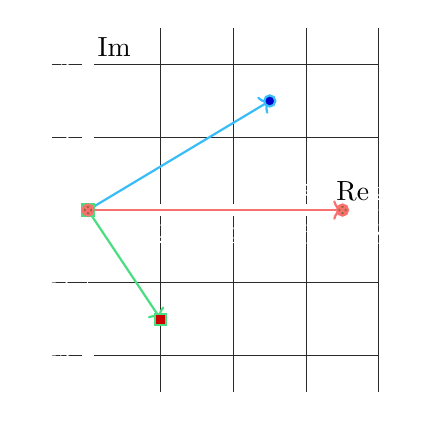
\begin{tikzpicture}
\begin{axis}[
  axis lines=middle, grid=both,
  xmin=-1, xmax=8, ymin=-5, ymax=5,
  width=0.78\linewidth, height=6.2cm,
  xlabel={Re}, ylabel={Im},
  axis equal image,
]
\VectorFromOrigin{5}{3}{z_1}
\addplot+[->, thick, color=green] coordinates {(0,0) (2,-3)};
\node[anchor=north west, text=text] at (axis cs:2,-3) {$z_2$};

\addplot+[->, thick, color=redacc] coordinates {(0,0) (7,0)};
\node[anchor=south, text=text] at (axis cs:7,0) {$z_1+z_2$};
\end{axis}
\end{tikzpicture}
\end{center}
\end{QAPair}

\begin{QAPair}{Q9(i-b) Graphical difference for $z_1=5+3i,\ z_2=2-3i$}
\textcolor{gold}{\bfseries Question:} Represent $z_1-z_2$ graphically for $z_1=5+3i$, $z_2=2-3i$.
\tcblower
\textcolor{green}{\bfseries Answer:}
\Step{1} Subtract:
\[
z_1-z_2=(5+3i)-(2-3i)=3+6i.
\]
\Step{2} Plot $z_1$ and $-z_2$, then the sum $z_1+(-z_2)$.
\begin{center}
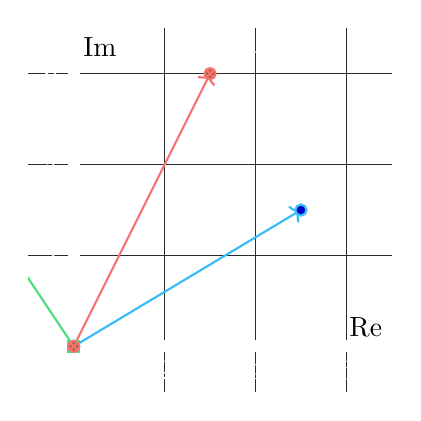
\begin{tikzpicture}
\begin{axis}[
  axis lines=middle, grid=both,
  xmin=-1, xmax=7, ymin=-1, ymax=7,
  width=0.78\linewidth, height=6.2cm,
  xlabel={Re}, ylabel={Im},
  axis equal image,
]
\VectorFromOrigin{5}{3}{z_1}
\addplot+[->, thick, color=green] coordinates {(0,0) (-2,3)};
\node[anchor=south east, text=text] at (axis cs:-2,3) {$-z_2$};

\addplot+[->, thick, color=redacc] coordinates {(0,0) (3,6)};
\node[anchor=south west, text=text] at (axis cs:3,6) {$z_1-z_2$};
\end{axis}
\end{tikzpicture}
\end{center}
\end{QAPair}

\begin{QAPair}{Q9(ii-a) Graphical sum for $z_1=-3+2i,\ z_2=-4+3i$}
\textcolor{gold}{\bfseries Question:} Represent $z_1+z_2$ graphically for $z_1=-3+2i$, $z_2=-4+3i$.
\tcblower
\textcolor{green}{\bfseries Answer:}
\[
z_1+z_2=(-3+2i)+(-4+3i)=\mathbf{-7+5i}.
\]
\begin{center}
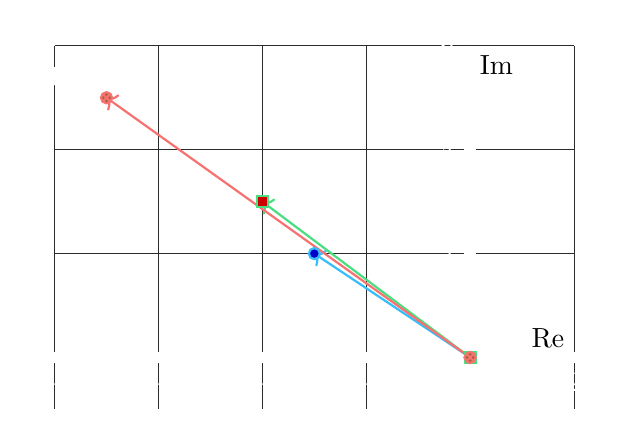
\begin{tikzpicture}
\begin{axis}[
  axis lines=middle, grid=both,
  xmin=-8, xmax=2, ymin=-1, ymax=6,
  width=0.78\linewidth, height=6.2cm,
  xlabel={Re}, ylabel={Im},
  axis equal image,
]
\addplot+[->, thick, color=cyan] coordinates {(0,0) (-3,2)};
\node[anchor=south east, text=text] at (axis cs:-3,2) {$z_1$};

\addplot+[->, thick, color=green] coordinates {(0,0) (-4,3)};
\node[anchor=south east, text=text] at (axis cs:-4,3) {$z_2$};

\addplot+[->, thick, color=redacc] coordinates {(0,0) (-7,5)};
\node[anchor=south east, text=text] at (axis cs:-7,5) {$z_1+z_2$};
\end{axis}
\end{tikzpicture}
\end{center}
\end{QAPair}

\begin{QAPair}{Q9(ii-b) Graphical difference for $z_1=-3+2i,\ z_2=-4+3i$}
\textcolor{gold}{\bfseries Question:} Represent $z_1-z_2$ graphically for $z_1=-3+2i$, $z_2=-4+3i$.
\tcblower
\textcolor{green}{\bfseries Answer:}
\[
z_1-z_2=(-3+2i)-(-4+3i)=\mathbf{1-i}.
\]
\begin{center}
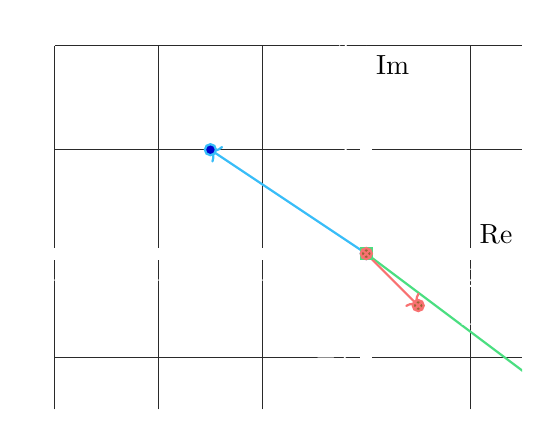
\begin{tikzpicture}
\begin{axis}[
  axis lines=middle, grid=both,
  xmin=-6, xmax=3, ymin=-3, ymax=4,
  width=0.78\linewidth, height=6.2cm,
  xlabel={Re}, ylabel={Im},
  axis equal image,
]
\addplot+[->, thick, color=cyan] coordinates {(0,0) (-3,2)};
\node[anchor=south east, text=text] at (axis cs:-3,2) {$z_1$};

\addplot+[->, thick, color=green] coordinates {(0,0) (4,-3)};
\node[anchor=north west, text=text] at (axis cs:4,-3) {$-z_2$};

\addplot+[->, thick, color=redacc] coordinates {(0,0) (1,-1)};
\node[anchor=north west, text=text] at (axis cs:1,-1) {$z_1-z_2$};
\end{axis}
\end{tikzpicture}
\end{center}
\end{QAPair}

% ============================================================
% Q10: product graphically (plot z1, z2, and product)
\begin{QAPair}{Q10(i) Product for $z_1=4+2i,\ z_2=-2+3i$}
\textcolor{gold}{\bfseries Question:} Represent the product graphically for $z_1=4+2i$ and $z_2=-2+3i$.
\tcblower
\textcolor{green}{\bfseries Answer:}
\Step{1} Multiply:
\[
(4+2i)(-2+3i)=-8+12i-4i+6i^2=-14+8i.
\]
So $z_1z_2=\mathbf{-14+8i}$.

\textcolor{gold}{\bfseries Plot (points $z_1,\ z_2,\ z_1z_2$)}\\
\begin{center}
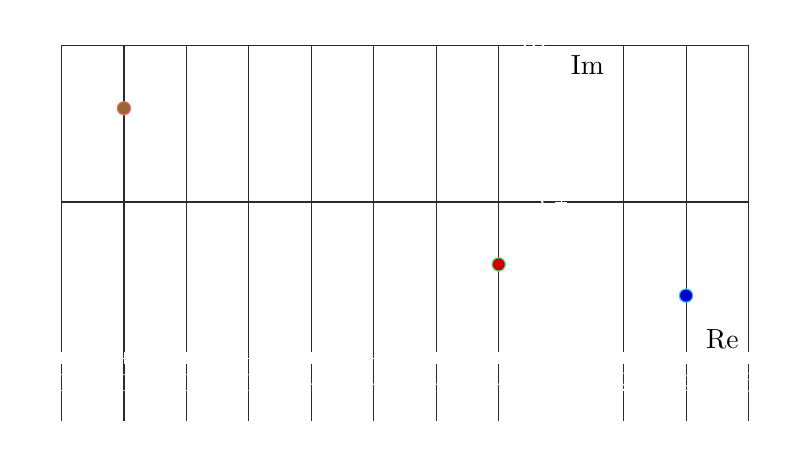
\begin{tikzpicture}
\begin{axis}[
  axis lines=middle, grid=both,
  xmin=-16, xmax=6, ymin=-2, ymax=10,
  width=0.85\linewidth, height=6.6cm,
  xlabel={Re}, ylabel={Im},
  axis equal image,
]
\addplot+[only marks, mark=*, mark size=2.4pt, color=cyan] coordinates {(4,2)};
\node[anchor=south west, text=text] at (axis cs:4,2) {$z_1$};

\addplot+[only marks, mark=*, mark size=2.4pt, color=green] coordinates {(-2,3)};
\node[anchor=south east, text=text] at (axis cs:-2,3) {$z_2$};

\addplot+[only marks, mark=*, mark size=2.4pt, color=redacc] coordinates {(-14,8)};
\node[anchor=south east, text=text] at (axis cs:-14,8) {$z_1z_2$};
\end{axis}
\end{tikzpicture}
\end{center}
\end{QAPair}

\begin{QAPair}{Q10(ii) Product for $z_1=2+4i,\ z_2=3-i$}
\textcolor{gold}{\bfseries Question:} Represent the product graphically for $z_1=2+4i$ and $z_2=3-i$.
\tcblower
\textcolor{green}{\bfseries Answer:}
\Step{1} Multiply:
\[
(2+4i)(3-i)=6-2i+12i-4i^2=10+10i.
\]
So $z_1z_2=\mathbf{10+10i}$.

\textcolor{gold}{\bfseries Plot (points $z_1,\ z_2,\ z_1z_2$)}\\
\begin{center}
\begin{tikzpicture}
\begin{axis}[
  axis lines=middle, grid=both,
  xmin=-1, xmax=12, ymin=-4, ymax=12,
  width=0.85\linewidth, height=6.6cm,
  xlabel={Re}, ylabel={Im},
  axis equal image,
]
\addplot+[only marks, mark=*, mark size=2.4pt, color=cyan] coordinates {(2,4)};
\node[anchor=south west, text=text] at (axis cs:2,4) {$z_1$};

\addplot+[only marks, mark=*, mark size=2.4pt, color=green] coordinates {(3,-1)};
\node[anchor=north west, text=text] at (axis cs:3,-1) {$z_2$};

\addplot+[only marks, mark=*, mark size=2.4pt, color=redacc] coordinates {(10,10)};
\node[anchor=south west, text=text] at (axis cs:10,10) {$z_1z_2$};
\end{axis}
\end{tikzpicture}
\end{center}
\end{QAPair}

% ============================================================
% Q11: division graphically
\begin{QAPair}{Q11(i) Represent $\dfrac{z_1}{z_2}$ for $z_1=6-4i,\ z_2=3$}
\textcolor{gold}{\bfseries Question:} Represent $z_1\div z_2$ graphically when $z_1=6-4i$, $z_2=3$.
\tcblower
\textcolor{green}{\bfseries Answer:}
\Step{1} Divide by real number $3$ (it scales both parts):
\[
\frac{6-4i}{3}=2-\frac{4}{3}i.
\]
So the quotient is $\mathbf{2-\frac{4}{3}i}$.

\textcolor{gold}{\bfseries Plot (quotient point)}\\
\PointPlot{q}{2}{-1.3333}{5}
\end{QAPair}

\begin{QAPair}{Q11(ii) Represent $\dfrac{z_1}{z_2}$ for $z_1=-4-6i,\ z_2=1+i$}
\textcolor{gold}{\bfseries Question:} Represent $z_1\div z_2$ graphically when $z_1=-4-6i$, $z_2=1+i$.
\tcblower
\textcolor{green}{\bfseries Answer:}
\Step{1} Use conjugate:
\[
\frac{-4-6i}{1+i}\cdot\frac{1-i}{1-i}
=\frac{(-4-6i)(1-i)}{(1+i)(1-i)}.
\]
\Step{2} Denominator:
\[
(1+i)(1-i)=1^2+1^2=2.
\]
\Step{3} Numerator:
\[
(-4-6i)(1-i)=-4+4i-6i+6i^2=-10-2i.
\]
\Step{4} Divide by $2$:
\[
\frac{-10-2i}{2}=\mathbf{-5-i}.
\]
\textcolor{gold}{\bfseries Plot (quotient point)}\\
\PointPlot{q}{-5}{-1}{6}
\end{QAPair}

\end{document}
